\documentclass{article}

\usepackage{amsmath,amssymb}
\usepackage{tikz}
\usepackage{pgfplots}
\usepackage{xcolor}
\usepackage[left=2.1cm,right=3.1cm,bottom=3cm,footskip=0.75cm,headsep=0.5cm]{geometry}
\usepackage{enumerate}
\usepackage{enumitem}
\usepackage{marvosym}
\usepackage{tabularx}

\usepackage[utf8]{inputenc}

\renewcommand*{\arraystretch}{1.4}

\newcolumntype{L}[1]{>{\raggedright\arraybackslash}p{#1}}
\newcolumntype{R}[1]{>{\raggedleft\arraybackslash}p{#1}}
\newcolumntype{C}[1]{>{\centering\let\newline\\\arraybackslash\hspace{0pt}}m{#1}}

\title{\textbf{Rechtfertigung der Staatstätigkeit, Hausaufgaben 1}}
\author{\textsc{Henry Haustein}}
\date{}

\begin{document}
	\maketitle
	
	\section*{Aufgabe 1}
	\begin{enumerate}[label=(\alph*)]
		\item Wenn $\bar{x}=0$, dann offensichtlich $x_1=x_2=0$ und somit $u_1=u_2=0$. Dies ist auch die einzig mögliche Allokation, also auch die optimale Allokation. Wenn $\bar{x}>0$, dann gilt $W=0$ nur dann, wenn $u_1=x_1=0$ und $u_2=x_2=\bar{x}$. In diesem Fall kommt es zu einer Wohlfahrtssteigerung, wenn man eine Verteilung wählt, bei der $x_1,x_2>0$ ist.
		\item Mit dem Lagrange-Ansatz folgt:
		\begin{align}
			L = x_1\cdot x_2 + \lambda(x_1+x_2-\bar{x}) \notag
		\end{align}
		Die Bedingungen erster Ordnung lauten:
		\begin{align}
			\label{1.1}
			\frac{\partial L}{\partial x_1} &= x_2 + \lambda = 0 \tag{1.1} \\
			\label{1.2}
			\frac{\partial L}{\partial x_2} &= x_1 + \lambda = 0 \tag{1.2}
		\end{align}
		Subtaktion von \eqref{1.1} und \eqref{1.2} liefert $x_1-x_2=0$, also $x_1=x_2$ und damit $x_1=x_2=\frac{\bar{x}}{2}$.
	\end{enumerate}

	\section*{Aufgabe 2}
	\begin{enumerate}[label=(\alph*)]
		\item Mittels Lagrange ergibt sich
		\begin{align}
			L = U_1 + U_2 + \lambda(I_1 + I_2 - 1000) \notag
		\end{align}
		Die Bedingungen erster Ordnung lauten:
		\begin{align}
			\label{2.1}
			\frac{\partial L}{\partial I_1} &= 4000-2I_1 + \lambda = 0 \tag{2.1} \\
			\label{2.2}
			\frac{\partial L}{\partial I_2} &= 4000-6I_2 + \lambda = 0 \tag{2.2}
		\end{align}
		Subtaktion von \eqref{2.1} und \eqref{2.2} liefert
		\begin{align}
			4000-2I_1 &= 4000-6I_2 \notag \\
			I_1 &= 3I_2 \notag \\
			I_1 &= 750 \notag \\
			I_2 &= 250 \notag
		\end{align}
		\item Graph
		\begin{center}
			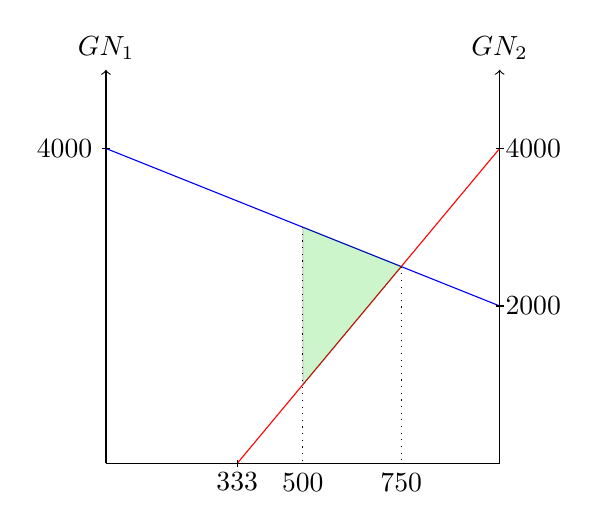
\begin{tikzpicture}
				\draw[->] (0,0) -- (0,5) node[above] {$GN_1$};
				\draw (0,0) -- (5,0);
				\draw[->] (5,0) -- (5,5) node[above] {$GN_2$};
				
				\draw[blue] (0,4) -- (5,2);
				\draw[red] (5,4) -- (5/3,0);
				
				\draw (0.05,4) -- (-0.05,4) node[left] {4000};
				\draw (5.05,4) -- (4.95,4) node[right] {4000};
				\draw (5.05,2) -- (4.95,2) node[right] {2000};
				\draw (5/3,0.05) -- (5/3,-0.05) node[below,yshift=1.5] {333};
				
				\draw[dotted] (15/4,2.5) -- (15/4,0) node[below] {750};
				\draw[dotted] (2.5,3) -- (2.5,0) node[below] {500};
				
				\draw[fill=green!80!black,opacity=0.2] (2.5,1) -- (2.5,3) -- (15/4,2.5) -- (2.5,1);
			\end{tikzpicture} \\
			\textcolor{blue}{$GN_1$}, \textcolor{red}{$GN_2$}, \textcolor{green!80!black}{Wohlfahrtsverlust}
		\end{center}
		Nimmt man Person 1 etwas weg und gibt es Person 2, so sinkt der sinkt der Grenznutzen von 1 nur ein bisschen, aber der Grenznutzen 2 steigt viel stärker. Eine solche Umverteilung kann man solange machen, bis sich die Grenznutzen angleichen.
	\end{enumerate}

	\section*{Aufgabe 3}
	\begin{enumerate}[label=(\alph*)]
		\item Das Budget ist $p_1x_1 + p_2x_2 = 2p_1 + 2p_2 = 2(p_1+p_2)$. Die Bugetgerade ist damit
		\begin{align}
			x_2 = \frac{2(p_1+p_2)}{p_2} - \frac{p_1}{p_2}x_1 \notag
		\end{align}
		\begin{center}
			\begin{tikzpicture}
			\begin{axis}[
			xmin=0, xmax=1, xlabel=$x_1$,
			ymin=0, ymax=1, ylabel=$x_2$,
			samples=400,
			axis x line=middle,
			axis y line=middle,
			domain=0:1,
			yticklabels={,,},
			xticklabels={,,},
			xtick style={draw=none},
			ytick style={draw=none},
			]
			\addplot[mark=none,smooth,blue] {0.9- 1.1111*x};
			
			\node at (axis cs: 0.3,0.9) (a) {$\left(0,\frac{2(p_1+p_2)}{p_2}\right)$};
			\node at (axis cs: 0.85,0.2) (b) {$\left(\frac{2(p_1+p_2)}{p_1},0\right)$};
			
			\draw[->,dotted] (a) to[bend right=10] (axis cs: 0,0.9);
			\draw[->,dotted] (b) to[bend left=10] ( axis cs: 0.81,0);
			
			\end{axis}
			\end{tikzpicture}
		\end{center}
		\item Wenn $p_1$ steigt, so verschieben sich die Achsenabschnitte und damit die Budgetgerade. So wird der Achsenabschnitt $\frac{2(p_1+p_2)}{p_2}$ größer werden, während $\frac{2(p_1+p_2)}{p_1}$ kleiner wird. Die Budgetgerade dreht sich also um den Punkt der Anfangsausstattung $(2,2)$.
		\begin{center}
			\begin{tikzpicture}
			\begin{axis}[
			xmin=0, xmax=1, xlabel=$x_1$,
			ymin=0, ymax=1, ylabel=$x_2$,
			samples=400,
			axis x line=middle,
			axis y line=middle,
			domain=0:1,
			yticklabels={,,},
			xticklabels={,,},
			xtick style={draw=none},
			ytick style={draw=none},
			]
			\addplot[mark=none,smooth,blue] {0.9- 1.1111*x};
			\addplot[mark=none,smooth,blue, dashed] {1- 1.5*x};
			
			\draw[dotted] (axis cs: 1000/3889,0) -- (axis cs: 1000/3889,2389/3889) -- (axis cs: 0,2389/3889);
			
			\end{axis}
			\end{tikzpicture}
		\end{center}
		\item Maximiere den Nutzen $U=\ln(x_1) + \ln(x_2)$ unter der Nebenbedingung $p_1x_1 + p_2x_2 \le 2(p_1+p_2)$. Der Lagrange-Ansatz ist $L=\ln(x_1) + \ln(x_2) - \lambda(p_1x_1 + p_2x_2 - 2(p_1+p_2))$.
		\begin{align}
			\frac{\partial L}{\partial x_1} &= \frac{1}{x_1} - \lambda p_1 = 0 \notag \\
			\frac{\partial L}{\partial x_2} &= \frac{1}{x_2} - \lambda p_2 = 0 \notag \\
			\frac{\partial L}{\partial\lambda} &= p_1x_1 + p_2x_2 - 2(p_1+p_2) = 0 \notag
		\end{align}
		Aus den ersten beiden Gleichungen erhält man $\frac{x_2}{x_1} = \frac{p_1}{p_2}$, also $x_2=\frac{p_1}{p_2}x_1$ bzw. $x_1 = \frac{p_2}{p_1}x_2$. Setzt man dies in die 3. Gleichung ein, so erhält man die Nachfrage für $x_1$
		\begin{align}
			p_1x_1 + p_2\left(\frac{p_1}{p_2}x_1\right) &= 2(p_1+p_2) \notag \\
			2p_1x_1 &= 2(p_1+p_2) \notag \\
			x_1 &= \frac{p_1 + p_2}{p_1} \notag
		\end{align}
		Bzw. die Nachfrage für $x_2$
		\begin{align}
			p_1\left(\frac{p_2}{p_1}x_2\right) + p_2x_2 &= 2(p_1+p_2) \notag \\
			2p_2x_2 &= 2(p_1+p_2) \notag \\
			x_2 &= \frac{p_1 + p_2}{p_2} \notag
		\end{align}
		\item Die Erstausstattung von Gut 1 steigt um $\Delta$ auf $2+\Delta$. Damit steigt auch das Budget auf $2(p_1+p_2) + p_1\Delta$. Der Lagrange-Ansatz ist $L=\ln(x_1) + \ln(x_2) - \lambda(p_1x_1 + p_2x_2 - 2(p_1+p_2) - p_1\Delta)$.
		\begin{align}
			\frac{\partial L}{\partial x_1} &= \frac{1}{x_1} - \lambda p_1 = 0 \notag \\
			\frac{\partial L}{\partial x_2} &= \frac{1}{x_2} - \lambda p_2 = 0 \notag \\
			\frac{\partial L}{\partial\lambda} &= p_1x_1 + p_2x_2 - 2(p_1+p_2) - p_1\Delta = 0 \notag
		\end{align}
		Die ersten zwei Gleichungen sind die selben wie bei (c), wir können also die Ergebnisse direkt für die Nachfragen nach $x_1$ und $x_2$ benutzen:
		\begin{align}
			p_1x_1 + p_2x_2 &= 2(p_1+p_2) + p_1\Delta \notag \\
			2p_1x_1 &= 2(p_1+p_2) + p_1\Delta \notag \\
			x_1 &= \frac{p_1+p_2}{p_1} + \frac{\Delta}{2} \notag
		\end{align}
		Die Nachfrage nach $x_1$ steigt also um $\frac{\Delta}{2}$. Für $x_2$ sieht es ähnlich aus:
		\begin{align}
			p_1x_1 + p_2x_2 &= 2(p_1+p_2) + p_1\Delta \notag \\
			2p_2x_2 &= 2(p_1+p_2) + p_1\Delta \notag \\
			x_2 &= \frac{p_1+p_2}{p_2} + \frac{p_1}{p_2}\frac{\Delta}{2} \notag
		\end{align}
		Die Nachfrage nach $x_2$ steigt also um das Preisverhältnis mal $\frac{\Delta}{2}$.
	\end{enumerate}

	\section*{Aufgabe 4}
	\begin{enumerate}[label=(\alph*)]
		\item Der Lagrange-Ansatz liefert (aus Gründen der Lesbarkeit lasse ich das $i$ vorerst weg)
		\begin{align}
			L = \sqrt{x_1} \cdot \sqrt{x_2} - \lambda(x_1p_1 + x_2p_2 - m) \notag
		\end{align}
		Die Bedingungen erster Ordnung lauten
		\begin{align}
			\frac{\partial L}{\partial x_1} &= \frac{\sqrt{x_2}}{2\sqrt{x_1}} -\lambda p_1 = 0 \notag \\
			\label{4.1}
			\frac{\sqrt{x_2}}{2\sqrt{x_1}} &= \lambda p_1 \tag{4.1} \\
			\frac{\partial L}{\partial x_2} &= \frac{\sqrt{x_1}}{2\sqrt{x_2}} -\lambda p_2 = 0 \notag \\
			\label{4.2}
			\frac{\sqrt{x_1}}{2\sqrt{x_2}} &= \lambda p_2 \tag{4.2}
		\end{align}
		Division von \eqref{4.1} durch \eqref{4.2} liefert
		\begin{align}
			\frac{\frac{\sqrt{x_2}}{2\sqrt{x_1}}}{\frac{\sqrt{x_1}}{2\sqrt{x_2}}} &= \frac{\lambda p_1}{ \lambda p_2} \notag \\
			\frac{\sqrt{x_2}\sqrt{x_2}}{\sqrt{x_1}\sqrt{x_1}} &= \frac{p_1}{p_2} \notag \\
			\label{4.3}
			x_2 &= \frac{p_1}{p_2}\cdot x_1 \tag{4.3}
		\end{align}
		Setzt man dies in die Budgetrestriktion ein, so ergibt sich
		\begin{align}
			m &= x_1p_1 + x_2p_2 \notag \\
			&= x_1p_1 + p_2\left(\frac{p_1}{p_2}\cdot x_1\right) \notag \\
			&= x_1p_1 + x_1p_1 \notag \\
			x_1 &= \frac{m}{2p_1} \notag
		\end{align}
		Einsetzen in \eqref{4.3} liefert
		\begin{align}
			x_2 &= \frac{p_1}{p_2} \cdot \frac{m}{2p_1} \notag \\
			&= \frac{m}{2p_2} \notag
		\end{align}
		Da die beiden Konsumenten die selbe Nutzenfunktion haben, gilt $x_1=x_1^A=x_1^B$ und $x_2=x_2^A=x_2^B$.
		\item Es gibt insgesamt 8 Einheiten von $x_1$ zu kaufen, also gilt:
		\begin{align}
			x_1^A + x_1^B &= 8 \notag \\
			\frac{m^A}{2p_1} + \frac{m^B}{2p_1} &= 8 \notag \\
			\frac{5p_1 + 3p_2}{2p_1} + \frac{3p_1 + 5p_2}{2p_1} &= 8 \notag \\
			\frac{5p_1 + 3}{2p_1} + \frac{3p_1 + 5}{2p_1} &= 8 \notag \\
			5p_1 + 3 + 3p_1 + 5 &= 8\cdot 2p_1 \notag \\
			8p_1 + 8 &= 16p_1 \notag \\
			p_1 + 1 &= 2p_1 \notag \\
			p_1 &= 1 \notag
		\end{align}
		\item Die gleichgewichtigen Konsummengen sind
		\begin{align}
			x_1^A &= \frac{5\cdot 1 + 3\cdot 1}{2\cdot 1} = 4 \notag
			x_2^A &= \frac{5\cdot 1 + 3\cdot 1}{2\cdot 1} = 4 \notag
			x_1^B &= \frac{3\cdot 1 + 5\cdot 1}{2\cdot 1} = 4 \notag
			x_2^B &= \frac{3\cdot 1 + 5\cdot 1}{2\cdot 1} = 4 \notag
		\end{align}
		\item Es ist zu zeigen, dass $GRS_A=GRS_B$ im Gleichgewicht gilt:
		\begin{align}
			GRS_A &= GRS_B \notag \\
			\frac{\sqrt{x_2^A}}{2\sqrt{x_1^A}} &= \frac{\sqrt{x_2^B}}{2\sqrt{x_1^B}} \notag \\
			\frac{\sqrt{4}}{2\sqrt{4}} &= \frac{\sqrt{4}}{2\sqrt{4}} \notag \\
			\frac{1}{2} &= \frac{1}{2} \notag
		\end{align}
		\item Edgeworth-Box mit Kontraktkurve und gesticheltem Preisverhältnis. Die Kontraktkurve zeigt alle pareto-optimalen Lösungen für den beidseitig optimalen Tausch.
		\begin{center}
			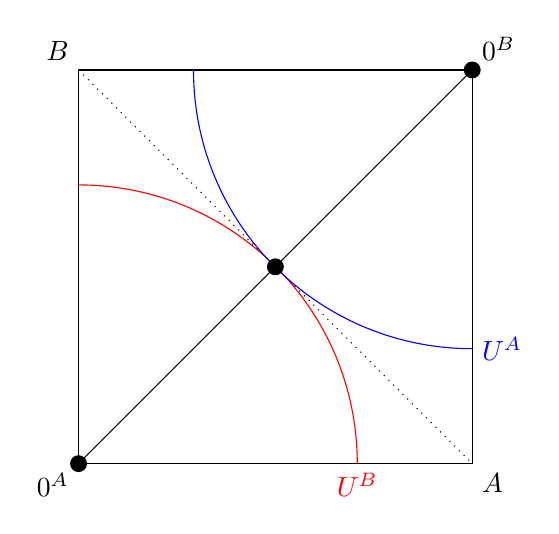
\begin{tikzpicture}
				\draw (0,0) rectangle (5,5);
				\draw[fill=black] (0,0) circle (0.1) node[below left] {$0^A$};
				\draw[fill=black] (5,5) circle (0.1) node[above right] {$0^B$};
				\node[above left] at (0,5) {$B$};
				\node[below right] at (5,0) {$A$};
				
				\draw[red] (0,3.54) arc (90:0:3.54) node[below] {$U^B$};
				\draw[blue] (1.46,5) arc (180:270:3.54) node[right] {$U^A$};
				
				\draw[dotted] (0,5) to (5,0);
				\draw (0,0) -- (5,5);
				
				\draw[fill=black] (2.5,2.5) circle (0.1);
			\end{tikzpicture}
		\end{center}
	\end{enumerate}

	\section*{Aufgabe 5}
	\begin{enumerate}[label=(\alph*)]
		\item Es ist der Gewinn $\Pi = p\cdot Y = 8\cdot \sqrt[4]{N}\cdot \sqrt[4]{K} - w\cdot N - r\cdot K = 8\sqrt{2}\cdot \sqrt[4]{K} - 4 - K$. Die Bedingung erster Ordnung lautet
		\begin{align}
			\frac{\partial \Pi}{\partial K} &= 8\sqrt{2}\cdot\frac{1}{4\sqrt[4]{K^3}} - 1 = 0 \notag \\
			\frac{2\sqrt{2}}{\sqrt[4]{K^3}} &= 1 \notag \\
			2\sqrt{2} &= \sqrt[4]{K^3} \notag \\
			64 &= K^3 \notag \\
			K^\ast &= 4 \notag
		\end{align}
		\item Die gewinnmaximierende Produktionsmenge ist dann $Y^\ast = \sqrt[4]{4} \cdot \sqrt[4]{4}=\sqrt{2}\cdot\sqrt{2} = 2$.
		\item Der Gewinn ist dann $\Pi^\ast = 8\cdot 2 = 16$.
	\end{enumerate}

	\section*{Aufgabe 6}
	\begin{enumerate}[label=(\alph*)]
		\item Der Lagrange-Ansatz liefert
		\begin{align}
			L &= rK + wN - \lambda(N^a\cdot K^b - \bar{Y}) \notag
		\end{align}
		Die Bedingungen erster Ordnung lauten
		\begin{align}
			\frac{\partial L}{\partial K} &= r-\lambda\cdot N^a\cdot b\cdot K^{b-1} = 0 \notag \\
			\lambda &= \frac{r}{N^a\cdot b\cdot K^{b-1}} \notag \\
			\frac{\partial L}{\partial N} &= w-\lambda\cdot K^b\cdot a\cdot N^{a-1} = 0 \notag \\
			w &= \frac{r}{N^a\cdot b\cdot K^{b-1}}\cdot K^b\cdot a\cdot N^{a-1} \notag \\
			w &= \frac{r\cdot a\cdot K}{b\cdot N} \notag \\
			\frac{K}{N} &= \frac{w}{r} \cdot\frac{b}{a} \notag
		\end{align}
		Das Faktoreinsatzverhältnis entspricht also dem Produkt des inversen Preisverhältnisses (teure Faktoren sollten wenig eingesetzt werden) und den Verhältnis der Effizienz (effiziente Faktoren sollten häufig eingesetzt werden)
		\item Die Isoquante gibt die Faktormengen an, die zum gleichen Output führen, während die Isokostengerade die Mengen angibt, die zu gleichen Kosten führen.
		\begin{center}
			\begin{tikzpicture}
				\begin{axis}[
					xmin=0, xmax=1, xlabel=$x$,
					ymin=0, ymax=1, ylabel=$y$,
					samples=400,
					axis x line=middle,
					axis y line=middle,
					domain=0:1,
					yticklabels={,,},
					xticklabels={,,},
					xtick style={draw=none},
					ytick style={draw=none},
					]
					\addplot[mark=none,smooth,blue] {0.75-x};
					\addplot[mark=none,smooth,red] {0.5/(2*x+0.5)};
					
					\draw[dotted] (axis cs: 0.25,0) -- (axis cs: 0.25,0.5) -- (axis cs: 0,0.5);
					
				\end{axis}
			\end{tikzpicture} \\
			\textcolor{blue}{Isokostengerade}, \textcolor{red}{Isoquante}
		\end{center}
		Am Tangentialpunkt dieser beiden Kurven kann man ein gegebenes Outputniveau zu minimalsten Kosten herstellen.
		\item Wir wissen
		\begin{align}
			\bar{Y} &= N^a\cdot K^b \notag \\
			&= N^a \cdot \left(N\cdot\frac{w}{r} \cdot\frac{b}{a}\right)^b \notag \\
			&= N^{a+b} \cdot \left(\frac{w}{r} \cdot\frac{b}{a}\right)^b \notag \\
			N^{a+b} &= \frac{\bar{Y}}{\left(\frac{w}{r} \cdot\frac{b}{a}\right)^b} \notag \\
			N^\ast &= \sqrt[a+b]{\frac{\bar{Y}}{\left(\frac{w}{r} \cdot\frac{b}{a}\right)^b}} \notag \\
			K^\ast &= N^\ast \cdot \frac{b}{a}\cdot\frac{w}{r} \notag \\
			&= \sqrt[a+b]{\frac{\bar{Y}}{\left(\frac{b}{a}\cdot\frac{w}{r}\right)^b}}\cdot\frac{b}{a}\cdot\frac{w}{r} \notag \\
			&= \sqrt[a+b]{\frac{\bar{Y}}{\left(\frac{b}{a}\cdot\frac{w}{r}\right)^a}} \notag
		\end{align}
	\end{enumerate}
	
\end{document}